\chapter{Introduction}
\label{introduction}
\section{Motivation}
The advent of the turbojet engine led to a transformation in both commercial and military aviation, allowing for much faster flight than previously possible with propellor-driven aircraft. 
However, the increased thrust of turbojets has come at great cost; significant acoustic radiation is generated by the rotating components (compressor, turbine, fan), by the combustion process, and ultimately by the free jet itself. 
On the commercial side, the escalating number of flights, encroachment of urban and residential areas near airports, and tightening of environmental regulations have combined to force airports to institute curfews, surcharges and flight path restrictions to combat noise pollution. 
For the military, hearing damage inflicted on nearby personnel (particularly flight deck crew on aircraft carriers) has necessitated the implementation of noise reduction concepts on tactical aircraft.
During takeoff and landing, when acoustic radiation is most problematic to ground crew and  surrounding urban and residential areas, the dominant noise source of the jet engine is the aeroacoustic radiation generated by the high velocity engine exhaust.
This has spurred extensive research, spanning over six decades, into the acoustic source mechanism in high speed, high Reynolds number jets. 

While progress has been made in the field of aeroacoustics, both experimentally \citep{Tam1996, Viswanathan2006, Tam2008} as well as theoretically \citep{Cabana2008}, understanding of jet noise sources and their radiation mechanisms remains incomplete \citep{Jordan2008}.
This is due to the large number of interrelated parameters (e.g. Reynolds number, temperature ratio, acoustic Mach number, nozzle geometry, et cetera) as well as the large disparity in the associated length and time scales of the turbulent phenomena and the radiated noise.
Simulations of controlled free shear layers have suggested that there is significant potential for noise reduction, on the order of 11 dB in some cases \citep{Wei2006}.
However, these simulations relied on non-physically defined actuation (that is, forcing was applied over a defined region by arbitrary energy, momentum, and body force terms), and a physical interpretation of the optimum forcing parameters was not immediately clear to the researchers.
Current noise-mitigation technologies for free jets have largely been applied in an adhoc fashion, due to our incomplete understanding of the aeroacoustic sources.
Fully realizing this maximum noise reduction potential will require a much more detailed understanding of the mechanism (or mechanisms) by which free jets radiate to the far-field.

It is generally agreed that the dominant noise sources are related to the large-scale turbulent structures present in the mixing layer of the jet. 
What remains to be determined is what aspects of the large-scale structure evolution and interactions are relevant to the noise generation process. 
Theoretical models of spatially- and temporally-modulated coherent structures have shown great promise in replicating the observed characteristics of the dominant far-field noise \citep{Cavalieri2010}. 
However, direct experimental data linking this structure evolution to the acoustic emission is still lacking. 
It is on this vein that the current work is focused.
Until recently, experimental data acquisition techniques have been unable to capture the flow physics with enough fidelity (lacking in either spatial or temporal resolution) in order to accurately model the large-scale structures and aeroacoustic sources.
By combining contemporary data acquisition methods (free-field microphones and non-time-resolved particle image velocimetry) with novel post-processing algorithms this work aims to directly link the relevant vortex dynamics of the large-scale structures to the acoustic emission events, and in the process identify a simplified aeroacoustic source mechanism. 

This study can be broken down into three distinct parts. 
In the first, the irrotational near-field and acoustic far-field of the jet is analyzed in order to identify the dominant acoustic source region.
In the second, time-resolved velocity fields are estimated using an artificial neural network, which is trained to generate a mapping from time-resolved pressure measurements to instantaneous velocity.
Lastly, the acoustic source is computed from the time-resolved velocity using Ribner's simplification of Lighthill's acoustic analogy.  
	
\section{Background}
\subsection{Flow Control}
\label{sec:flow_instabilities}
Controlling the development of the jet plume, and hence controlling the rate of mixing or intensity and characteristics of the emitted acoustic radiation, is a long running goal of the aeroacoustic community.
Passive, permanent modifications to the nozzle have been shown to be quite adept at this task; some examples of these include tabs or chevrons \citep{Bridges2004}. 
These work to generate counter-rotating streamwise vortices in the developing shear layer, which serve to substantially increase mixing between the core and coflow in the near-nozzle region and ultimately retard the growth of large-scale axisymmetric structures \citep{Samimy1993}.

Unfortunately, these passive modifications have associated penalties to the engine performance, in terms of added weight or reduced thrust.
Due to the passive nature of the flow modification, these performance penalties are in effect over the entire duration of the flight regardless of whether or not the noise reduction is needed. 
To improve engine efficiency, active control techniques are desired, since they can be activated when needed, such as during takeoff and landing, and deactivated when unneeded, such as after a commercial airliner reaches cruising altitude. 
Active control techniques, which seek to manipulate instabilities in the jet shear layer, have been extensively studied in low-speed, low-Reynolds number jets, the most common of which is acoustic drivers. 
However, as the speed and Reynolds number of the jet is increased (to match those in practical applications), so too does the required bandwidth and energy of the active drivers. 
Hence, acoustic or magneto-hydrodynamic drivers lose control authority in these regimes, and more powerful actuators are required.

The last decade has seen a rapid growth in the development of plasma actuators for use in high-speed flow control; though as of yet they have not progressed past the experimental phase.
Localized arc filament plasma actuators (LAFPAs) are one such class of plasma actuator, which were developed by a collaboration between the Gas Dynamics and Turbulence Laboratory (GDTL) and the Non-Equilibrium Thermodynamics Laboratory (NETL) at the Ohio State University.
LAFPAs can provide the high-amplitude and high-frequency excitation required for control of high Mach number and high Reynolds number jets \citep{Utkin2007}. 
GDTL has used these actuators for noise mitigation and flow control in Mach 0.9, Mach 1.3 and Mach 1.65 jets (both heated and unheated) \citep{Samimy2007,Samimy2007a,Samimy2010,Kim2011,Kim2009,Kearney-Fischer2009}. 
A review of the development of LAFPAs and their use in flow control and fluid phenomena research in high speed, high Reynolds number jets can be found in Samimy \etal \citep{Samimy2012}. 
More recently, the diagnostic potential of LAFPAs for understanding jet flow phenomena has been explored. 
Excitation of instabilities in the flow by LAFPAs results in a definitive spatio-temporal origin to which resulting phenomena can be referenced. 
The absolute temporal reference afforded by LAFPA excitation provides researchers the ability to investigate the growth, saturation, and decay of structures with high fidelity. 
An example of their diagnostic potential can be found in the work of Kearney-Fischer \etal \citep{Kearney-Fischer2011a}, which investigated Mach wave radiation from heated, high Mach number jets using schlieren imaging phase-locked to LAFPAs. 

Unlike their passive counterparts (such as tabs or mechanical chevrons), or some other potential active flow control technologies (such as fluidic chevrons), LAFPAs control the shear layer development indirectly by exciting naturally occurring instabilities.
The sharp velocity gradient in the jet shear layer (or, more precisely the inflection point produced by this sharp gradient) gives rise to the inviscid Kelvin-Helmholtz instability \citep{Michalke1984} (sometimes simply referred to as the initial shear layer instability).
This instability is broadband and scales with the local momentum layer thickness and jet exit velocity ($\theta / U_j$) ; perturbations over a wide range of frequencies can be amplified, though the dominant frequencies are found to be on the order of $St_{\theta} = f \theta /U_j = 0.012$ for very thin boundary layers \citep{Cohen1987}. 
The Kelvin-Helmholtz instability then drives the development of the large-scale structures in the shear layer by amplifying fine-scale perturbations, ultimately causing them to roll-up into coherent structures regardless of Reynolds number \citep{Crow1971,Brown1974}.
Owing to the axisymmetry of the jet nozzle (i.e. that the initial shear layer wraps around and connects to itself), various azimuthal Fourier modes are unstable to perturbations (including both axisymmetric and higher order modes) \citep{Cohen1987}.

The growth of the shear layer as it advects downstream ultimately dictates that the shear layer merges with itself; this location is referred to as the end of the potential core.
A secondary instability, the jet column instability, manifests in axisymmetric jets and is related to the passage of large-scale structures through the end of the potential core.
This instability scales with the jet exit diameter and jet exit velocity ($D / U_j$) and is broadband, with a dominant characteristic frequency of $St_{D} = f D /U_j = 0.3$.
The relation of the jet column instability to the initial shear layer instability is not well understood.  
Kibens argued that the jet preferred frequency is related to the initial shear layer frequency by the number of pairings of large scale structures that occur before the end of the potential core (i.e. $f_n / f_p = 2^n$), as the frequency of the structures halves after each pairing process \citep{Kibens1980}.  
Conversely, Petersen claims that the jet preferred mode is simply the initial shear layer instability at the end of the potential core, and that the appearance of a single dominant lengthscale for the axisymmetric mode is due not to a type of `global' instability of the flow field, but to a cutoff at the end of the potential core of the axisymmetric instability \citep{Petersen1988}.
Regardless, it is clear that the large-scale oscillations of the jet shear layer and potential core are ultimately the product of small-scale perturbations which are amplified by the initial shear layer instability.

LAFPAs achieve flow control by utilizing this relationship between the initial shear layer instability and the jet column instability.
The localized plasma arc-filament produces a rapid, localized heating through the Joule effect, and a compression wave is formed \citep{Utkin2007}.
Though these perturbations are spatially discrete, they quickly amplify into large-scale coherent structures with well-defined characteristic spatial, temporal, and azimuthal frequencies.
Thus, LAFPAs are able to control the development of the most energetic scales in the jet shear layer; large-scale, azimuthally-coherent structures can be generated when enhanced mixing and jet spreading are desired, or smaller-scale, less azimuthally-coherent structures when noise reduction is necessary. 
In the present work, the subsonic jet is excited by LAFPAs, though here the goal is diagnostic rather than immediate practical application.
The well-defined frequencies and phase of the large-scale structures produced by LAFPA actuation serve as an excellent reference for data acquisition and post-processing (e.g. phase-locking and phase-averaging).

\subsection{Lighthill's Acoustic Analogy}
Far outside the jet, where the medium is quiescent, no sources or sinks are present, and any disturbances are low-amplitude and isentropic, the governing equations can be linearized and simply reduced to a homogeneous wave equation
\begin{equation}
	\frac{\partial^2 p}{\partial t^2} - c^2 \nabla ^2 p = 0
\end{equation}
which describes the non-dispersive propagation of (acoustic) waves through space and time.
Lighthill \citep{Lighthill1952} was the first to identify that the governing equations for fluid dynamics could also be rearranged in such a manner as to produce a propagating wave equation \textit{inside the jet}.
Prior to this, aeroacoustic studies had observed that the frequency content of the far acoustic field matched that of the flow field, but had not identified a way to estimate the acoustic intensity.

Starting with the conservation of mass and momentum equations, one can take the divergence of the former and the partial derivative with respect to time of the latter, and combine these along with the equation of state to produce
\begin{equation}
\frac{1}{c^2}\frac{\partial^2 p}{\partial t^2} - \nabla^2 p = \nabla \cdot \nabla \cdot \mathbf{T}.
\label{eq:lighthill_analogy}
\end{equation}
$\mathbf{T}$, commonly referred to as \textit{Lighthill's stress tensor}, comprises Reynolds stresses, viscous stresses, and entropy fluctuations, respectively:
\begin{equation}
\mathbf{T} = \rho \mathbf{u} \otimes \mathbf{u} - \mathbf{\tau} + \mathbf{I} \left[ (p-\bar{p}) - c^2 (\rho - \bar{\rho}) \right].
\end{equation}
Here, $c$ refers to the ambient speed of sound, $\mathbf{I}$ is the identity matrix, $\mathbf{\tau}$ is the shear stress tensor, and an overbar ($\bar{\cdot}$) corresponds to a time-averaged quantity.
This transformation has the effect of approximating the real system as a uniform acoustic medium at rest which is being driven by an external fluctuating force field.
As the wave operator is linear, the solution to this equation can be formulated with the aid of Green's functions,
\begin{eqnarray}
\frac{\partial^2 G}{\partial t^2} - c^2 \nabla^2 G = \delta (\tau -t) \delta (\mathbf{x}' - \mathbf{x}).
\end{eqnarray}
The solution to this (see Crighton \etal \citep{Crighton1992}) is the deceptively simple spatial integration of the source field at retarded time (that is, it is accounting for the propagation delay from the source location to the observer):
\begin{equation}
p (\mathbf{x},t) = \frac{1}{4 \pi c^2} \nabla \cdot \nabla \cdot \int_{\Omega} \frac{\mathbf{T} (\mathbf{x}',t - |\mathbf{x} - \mathbf{x}'|/c)}{|\mathbf{x} - \mathbf{x}'|} d^3 \mathbf{x}'.
\label{eq:source_integration}
\end{equation}

Lighthill's derivation of what became known as the first acoustic analogy (which in fact was specifically tailored to the study of jet noise) reformed the study of aeroacoustics.
As has been discussed by many authors before (see Goldstein \citep{Goldstein1974} for example), this equation describes the propagation of sound, through a quiescent medium, generated by quadrupole sources. 
There have been several major assumptions made in this derivation, that the flow is completely subsonic (and hence no shock or expansion waves are present), that the observer location is far from the jet (and hence hydrodynamic pressure fluctuations or `pseudo-sound' is negligible), that there are no solid boundaries near the flow (and hence, no reflections, diffraction, absorption, or scattering) and finally that the acoustic waves themselves do not act as sources as they propagate through the flow.
Nonetheless, this theoretical framework is still applicable to a wide variety of commercial and scientific inquiries, present study included.

Theoretical work based on Lighthill's approach was successful in predicting some aspects of experimentally-observed jet noise.
Namely, stochastic source models of quadrupoles (per the aeroacoustic community's understanding of jet turbulence at the time) predicted a far-field pressure intensity scaling of $I \sim U_{j}^{8}$ which agreed with experimental results from cold, subsonic jets at sideline angles \citep{Viswanathan2006}.
However, this scaling law does not hold when the jet is heated, necessitating more complex source models. 
Unfortunately, given the complexity of the source field, even modern experimental techniques cannot acquire the full source with sufficient spatial and temporal fidelity to elucidate the flow structures responsible for the dominant noise emission.

Later researchers further refined Lighthill's approach (e.g. Howe [cite], Goldstein \citep{Goldstein1974} and Lilley \citep{Lilley2003}); providing successively clearer characterizations of the source physics.
In addition to the true noise sources, Lighthill's acoustic source term includes flow-acoustic interactions, which describe diffraction and convection effects rather than true sources of noise, and which these researchers have attempted to separate from the true noise sources.
Alternative acoustic analogies have also been proposed, such as Powell's theory of vortex sound \citep{Powell1964} and Doak's momentum potential theory \citep{Doak1989}.
In a slightly different vein, analytical decompositions have been performed in order to separate the disparate fluid phenomena inherent in Lighthill's source term and identify the roles of each \citep{Cabana2008}.
In each of these theories however, the source field for a high-speed, turbulent jet is highly complex and defies a simple physical understanding of the dynamical processes which lead to the noise emission.   

\subsection{The Role of Large-Scale Structures}
Initial understanding of turbulence was that it was stochastic in nature - that the frequency and appearance of turbulent eddies in a flow was random, with little to no prescribed preference.
It was in this context that Lighthill's acoustic analogy was first developed, and as a result initial models for the source field assumed a stochastic distribution of quadrupoles.
This source model was shown to produce an intensity which scaled with the eighth-power of the flow velocity, which was in general agreement with the experimentally-observed intensity scaling of cold, subsonic jets \citep{Lighthill1954}.
The downstream convection of these quadrupoles produces a preferential directivity in the emitted acoustic radiation, with a maximum predicted to occur near 45$^\circ$ from the jet axis, again in general agreement of experimental far-field spectra \citep{Lighthill1954}.
However, researchers have found that stochastic quadrupole source models fail to accurately predict the intensity scaling of jet noise in heated jets or cold jets at low observer angles \citep{Tam1996}.
As Lighthill's analogy is an exact rearrangement of the governing equations (aside from the relatively minor assumption of a constant speed of sound), the error lies in our understanding of the aeroacoustic source. 

Mollo-Christensen \citep{Mollo-Christensen1967}, and later Crow \& Champagne \citep{Crow1971} and Brown \& Roshko \citep{Brown1974}, were the first to identified large-scale, coherent vortical structures underpinning turbulent free shear layers, in addition to the fine-scale, stochastic eddies.
Later researchers linked the appearance of these large-scale structures to natural flow instabilities (predominantly the Kelvin-Helmholtz instability discussed in \sect{sec:flow_instabilities}) \citep{Michalke1965,Michalke1984,Cohen1987}.
Following the identification these coherent structures in turbulent jet shear layers, source term models based on large-scale eddies have frequently been employed, to varying degrees of success. 

A simplified model of the noise generation process in stationary free jets can be found in \fig{fig:jet_sources_diagram}. 
This model is from the work of Tam \etal \citep{Tam1996, Tam2008}, who observed that the far-field spectra could be represented as a combination of two similarity spectra based on polar angle of the observer, regardless of jet Mach number or temperature.
At observer angles close to the jet downstream axis, the spectra exhibited a clearly defined spectral peak (\emph{F}-spectrum), whereas at sideline or upstream angles the spectra were broadband (\emph{G}-spectrum).
From this observation the two-component acoustic source model was born: the isotropic fine-scale turbulence, dominant in the near-nozzle region, is responsible for the omni-directional acoustic radiation that dominates the sideline and upstream polar angles. 
On the other hand, the large-scale turbulent structures which exist further downstream produce the superdirective radiation that is readily apparent at aft polar angles. 
This model of large-scale (and to a lesser extent fine-scale) turbulence noise generation explains the so-called 'mixing noise' generated by both subsonic and supersonic jets.
\begin{figure}
	\centering
	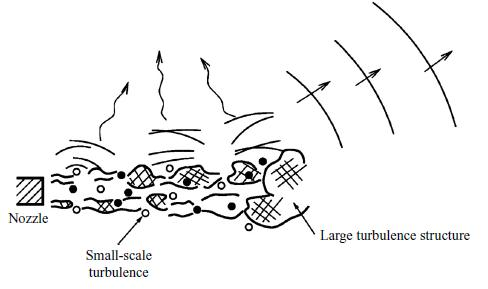
\includegraphics[width=5in]{Figures/JetNoiseSourceDiagramTMP.jpg}
	\caption{Simplified diagram of jet noise sources, reprinted from Tam \etal \citep{Tam2008a}.}
	\label{fig:jet_sources_diagram}
\end{figure}
Numerous experimental studies have lent credibility to this view of aeroacoustic noise generation; see for example, Panda \etal \citep{Panda2005}, Viswanathan \etal \citep{Viswanathan2010}, Tam \etal \citep{Tam2008}, and Bogey \& Bailley \citep{Bogey2007}.
There is little disagreement at this point that the large-scale coherent structures in the turbulent shear layer are responsible for the dominant noise emission; however, the exact dynamics of these which leads to acoustic emission are as of yet still not well-understood. 

As discussed by Tam \etal \citep{Tam1995} (among many others), large-scale structures can be represented as instability waves superimposed upon the mean flow.
At subsonic convection velocities, a plane instability wave with fixed frequency-wavenumber will emit no acoustic radiation to the far-field.
However, modulation of the instability wave's amplitude creates a dispersion in the energy content of the instability wave.
By doing so, the broadband instability wave, now commonly referred to as a \emph{wavepacket}, can shift energy to supersonic phase-velocities and hence produce sound.
Wavepacket models for noise emission have become commonplace, owing to their great success at predicting low-angle acoustic emission \citep{Obrist2011}.
Simple linear wavepacket models have allowed researchers to probe different aspects of the waveform modulation, in turn illuminating possible relevant dynamical behavior of the large-scale structures for the noise generation process.
Temporal modulation of the wavepacket's amplitude and spatial extent (termed `jittering' by the researchers) were shown to increase the efficiency of the noise source \citep{Cavalieri2010}; this conforms to experimental results which have indicated that the noise generation in free jets is highly intermittent \citep{Hileman2005,Kearney-Fischer2013}. 
Though progress has been made in experimentally measuring wavepacket characteristics in high-speed turbulent jets \citep{Cavalieri2013,Baqui2014}, a direct link between large-scale structure dynamics and the aeroacoustic source has remained elusive.
 
As a side note, additional noise source mechanisms have been identified for supersonic jets. In imperfectly expanded jets, shock cells are produced in the jet. As turbulent structures pass through these waves, the sharp pressure gradients cause them to emit acoustic radiation. 
This is observed directly in the far-field as a broad-band amplification at high frequencies, referred to simply as broad-band shock-associated noise (BBSAN). 
In stationary or subsonic airframes this radiation can generate a feedback loop, whereby the noise travels upstream to the nozzle exit, excites the initial shear layer, and produces new structures at the same frequency.
A high-amplitude, narrow-band tone (screech noise) is the end result of this feedback loop.
Lastly, supersonically-convecting (relative to the ambient) large-scale structures (which exist in supersonic and heated jets) produce high-amplitude, strongly-directional acoustic radiation towards aft angles.
This Mach wave radiation can be explained by a wavy-wall analogy \citep{Tam1995}.
In the present work, the jet is unheated and subsonic; as such these noise sources are not present and therefore neglected throughout the rest of this work.

 